\chapter{Элементарная работа силы и ее аналитическое выражение. Работа силы на
конечном пути. Работа равнодействующей. Мощность.}

\section{Элементарная работы силы и её аналитическое выражение}
Для характеристики действия, оказываемого силой на тело при некотором его 
перемещении, введём понятие о работе силы. Для этого введём понятие об 
элементарной работе.

\emph{Элементарной работой} силы \( \vec{F} \), приложенной в точке 
\( M \) (рис. \ref{pic51_01}), называется скалярная величина
\[ dA = F_\tau ds \quad (51.1) \]
где \( F_\tau \) -- проекция силы \( \vec{F} \) на касательную \( M\tau \) 
к траектории точки M, направленную в сторону перемещения этой точки 
(или проекция \( \vec{F} \) на направление скорости \( \vec{v} \) точки 
\( M \)); \( ds \) -- модуль элементарного перемещения точки \( M \).

\begin{figure}[h!]
    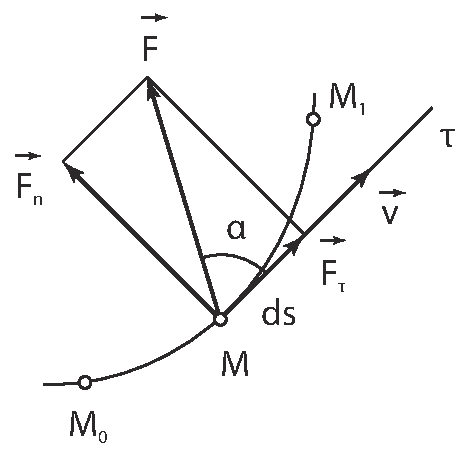
\includegraphics[width=.47\textwidth]{51_01}
    \parbox{.47\textwidth}{\caption{} \label{pic51_01}}
\end{figure}

Такое определение соответствует представлению о работе как о мере того 
действия силы, которое приводит к изменению модуля скорости точки. Если 
разложить силу \( \vec{F_\tau} \) на составляющие \( \vec{F_\tau} \) и 
\( \vec{F_n} \), то изменять модуль скорости будет \( \vec{F_\tau} \), 
так как \( F_\tau = ma_\tau = m\cdot dv/dt \).

Замечая, что \( F_\tau = F\cos\alpha \), где \( \alpha \) -- угол между 
\( \vec{F} \) и \( M\tau \), получим из (1) другое выражение для \( dA \):
\[ dA = Fds\cos\alpha \]

Если учесть, что \( ds = |d\vec{r}| \), где \( d\vec{r} \) -- вектор 
элементарного перемещения точки, и воспользоваться известным из векторной 
алгебры понятием о скалярном произведении двух векторов, то последнее 
равенство можно представить в виде:
\[ dA = \vec{F}\cdot d\vec{r} \]

Следовательно, \emph{элементарная работа силы равна скалярному произведению 
силы на вектор элементарного перемещения точки и её приложения.}

Если выразить скалярное произведение через проекции векторов \( \vec{F} \) 
и \( \vec{r} \) на координатные оси и учесть, что 
\( r_x = x, r_y = y, r_z = z \), то получим \emph{аналитическое выражение 
элементарной работы}
\[ dA = F_x dx + F_y dy + F_z dz \]
в котором \( x, y, z \) -- координаты точки приложения силы \( \vec{F} \).

\section{Работа силы на конечном пути}
Работа силы на любом конечном перемещении \( M_0 M_1 \) (рис. \ref{pic51_01}) 
вычисляется как предел интегральной суммы соответствующих элементарных 
работ 
\[ A_{(M_0 M_1)} = \int_{(M_0)}^{(M_1)} F_\tau ds \]
или 
\[ 
    A_{(M_0 M_1)} = \int_{(M_0)}^{(M_1)} 
    \left( F_x dx + F_y dy + F_z dz \right)
\]

Следовательно, \emph{работа силы на любом перемещении \( M_0 M_1 \) равна 
взятому вдоль этого перемещения интегралу от элементарной работы.}

Единицей измерения работы является в СИ -- 1 джоуль 
(1 Дж = 1 Н\( \cdot \)м = 1 кг \( \cdot\text{м}^2/\text{с}^2 \)).

\section{Работа равнодействующей}
Работа, совершенная равнодействующей силой равна алгебраической сумме 
работ, совершенных отдельными силами.
\[ A = \sum_{i=1}^{N} A_i \]

\section{Мощность}
Мощностью называется величина, определяющая работу, совершаемую силой 
в единицу времени. Если работа совершается равномерно, то мощность 
\( N = A/t_1 \), где \( t_1 \) -- время, в течении которого произведена 
работа \( A \). В общем случае
\[ N = \frac{dA}{dt} = F_\tau \frac{ds}{dt} = F_\tau v \]

Следовательно, \emph{мощность равна произведению касательной 
составляющей силы на скорость.}

Единицей измерения мощность в СИ является ватт (1 Вт = 1 Дж/с).

\newpage
